\section{Implementierung}

\begin{frame}{Benötigte Technologie}

Hardware:
\begin{itemize}
\item Physischer Server notwendig
\end{itemize}

Software:
\begin{itemize}
\item Tomcat Server (Webserver)
\item MySQL Server (Datenbankserver)
\item Tatsächliche Anwendung
\end{itemize}

Frameworks:
\begin{itemize}
\item Spring Boot (Container)\\
\item Thymeleaf (Templating)
\item Hibernate (Persistence)
\end{itemize}

\end{frame}


\begin{frame}{Authentifizierung}

\begin{itemize}
\item Nötig für Datensicherheit
\item Anhand von User-Daten wird Stauraum für Produkt ermittelt

\end{itemize}

\end{frame}


\begin{frame}{Showcase}

\begin{figure}
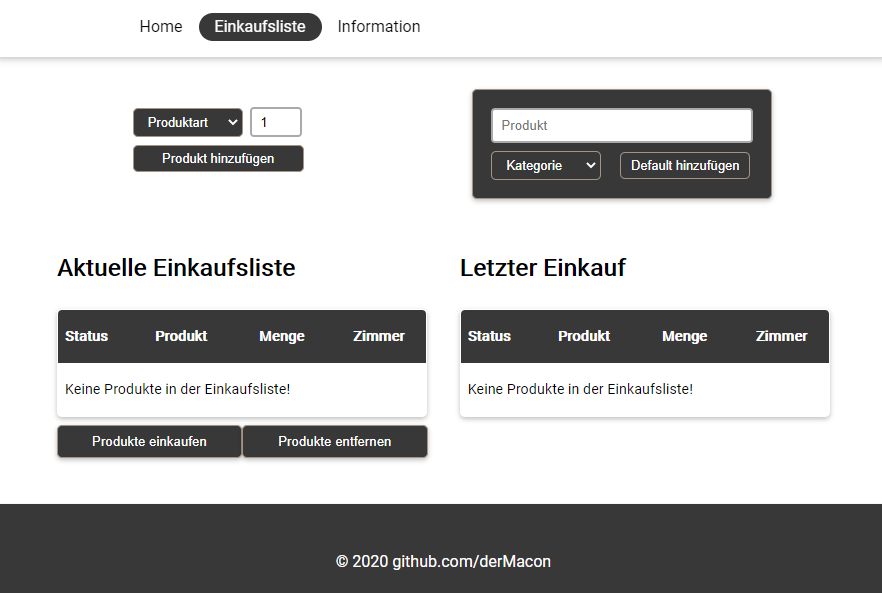
\includegraphics[width=.9\linewidth]{./_img/screenshot_01}
\end{figure}

\end{frame}






\begin{frame}{Roadmap}

Unmittelbar:
\begin{itemize}
\item Adminbereich einführen (neue Nutzer, etc.)
\item Darstellung aufräumen (Bootstrap, etc.)
\end{itemize}

Mittelfristig:
\begin{itemize}
\item Handyapp für Einkäufer
\begin{itemize}
\item REST Service notwendig (Client-Authentification)
\end{itemize}
\end{itemize}

Langfristig:
\begin{itemize}
\item Forum für Protokolle der WG-Treffen
\item Archiv über Stauräume im Haus
\end{itemize}

\end{frame}
